\subsection{精确求和、Monte Carlo 与非负估计的代价}

若 teacher forward 能提供该前缀完整 logits，则使用完整 $q$ 权重直接求式~\eqref{eq:center-expanded-k}，不需要生成第二条 response。信号在 log 空间用 logaddexp 计算，避免先形成极大的 $T/q$。该中心可以按 prefix 缓存并冻结。

若采用独立 $a_i\sim q(\cdot\mid s)$，有无偏估计
\begin{equation}
 \widehat K=-\frac1M\sum_{i=1}^MA(a_i),\qquad
 \Var\widehat K=V/M.
\end{equation}
$\widehat K$ 单次可以为负；这不违背其非负期望。另一个逐样本非负无偏估计为
\begin{equation}
 \widehat K_+=\frac1M\sum_i[\rho(a_i)-1-A(a_i)].
\end{equation}
两者期望相同，方差一般不同。 它们在局部与最坏尾部上具有不同表现。若 $\rho=1+\epsilon h$、$\E_qh=0$ 且 $h$ 有界，令 $c_0=1-\kappa(1-\eta)$，则
\begin{align}
 -A&=-\epsilon h+\tfrac12c_0\epsilon^2h^2+O(\epsilon^3),\\
 \phi(\rho)&=\tfrac12c_0\epsilon^2h^2+O(\epsilon^3),\\
 \Var(-A)&=\epsilon^2\E_qh^2+O(\epsilon^3),\\
 \Var\phi(\rho)&=\tfrac14c_0^2\epsilon^4\Var_q(h^2)+O(\epsilon^5).
\end{align}
因此包括 $\kappa=0$ 在内，接近同分布时非负控制变量估计可把方差从二阶降至四阶；这需要概率比一致接近一，不能扩展到任意重尾输入。

取 $q=(\epsilon,1-\epsilon)$、$T=(1/2,1/2)$、固定 $\kappa>0,\eta<1$，原始估计方差按 $O(\epsilon\log^2(1/\epsilon))\to0$；非负估计的稀有项为 $\rho\sim1/(2\epsilon)$，其方差按 $1/(4\epsilon)$ 发散。这个 $\rho-1$ 控制变量保证非负性，却不能提供统一低方差保证。固定数据上也可能降低方差，应记录真实条件矩后判断。 即便原 KL 很小，也不能自动使用局部结论：取 $q=(\epsilon,1-\epsilon)$、$T=(\epsilon^{1/4},1-\epsilon^{1/4})$，有 $\KL(q\Vert T)\sim\epsilon^{1/4}\to0$，但非负估计的方差按 $\epsilon^{-1/2}$ 发散。概率比一致接近一比 KL 小更强。

如果独立中心估计与当前 action 独立，$\Var[A(a)+\widehat K]=V+V/M$。估计中心不会自动降低标量 advantage 方差。若中心与 advantage 使用同一组 $M$ 个 action，固定参数下
\begin{equation}
 \E\left[\frac1M\sum_i(A_i-\bar A)\psi_i\right]
 =\frac{M-1}{M}\operatorname{Cov}_q(A,\psi).
\end{equation}
这个恒等式由展开双重和得到：$M$ 个同索引项贡献 $\E A\psi$，$M(M-1)$ 个异索引项贡献 $\E A\E\psi$。$M=1$ 时更新为零。 若同一个 action 改用非负估计 $\widehat K_+=\rho-1-A$，则
\begin{equation}
 A(a)+\widehat K_+(a)=\rho_a-1,
\end{equation}
完全消掉 $\kappa,\eta$ 的教师信号形状。在 $p=q$ 时，该 score 更新的期望是 $\E_T\psi_q$，对应 forward-KL 的下降方向，而不是原 $\E_qB\psi_q$。中心估计本身无偏，不代表与当前 action 共享样本后的梯度无偏。

$M>1$ 可以使用独立中心、leave-one-out 或无偏样本协方差系数；它们要求同一 prefix 下的独立动作，不能用不同前缀的 token 直接代替。本研究的主 BPO 路线采用完整条件求和，不引入 response 组。
\subsection{有界非负无偏中心估计器}

$q$ 提案下的非负估计会出现重尾，但可以利用已有 $K$ 上界构造另一个提案。令 $\kappa>0,\eta<1$，$c=-\log(1-\eta)/(\kappa\eta)\ge1$。由 $A\ge-c$ 与 $\phi\ge0$，逐 action 有
\begin{equation}
 0\le q_a\phi(\rho_a)\le T_a+(c-1)q_a.
\end{equation}
右侧的总质量是 $c$，所以定义归一化包络提案
\begin{equation}
 \mu_c=(1-1/c)q+(1/c)T,\qquad
 Z(a)=\frac{q_a}{\mu_c(a)}\phi(\rho_a),\quad a\sim\mu_c.
 \label{eq:center-bounded-mixture-estimator}
\end{equation}
无需知道真实 $K$ 即可采样：以概率 $1/c$ 从教师抽一个 action，否则从锚点抽一个 action。它只估计本 prefix 的中心，不把 response rollout 改为这个提案，也不引入 response 组。

\begin{theorem}[中心估计的最小统一样本上界]
\label{thm:center-bounded-estimator}
上述估计器满足
\begin{equation}
 \E_{\mu_c}Z=K,\qquad0\le Z\le c,\qquad
 \Var_{\mu_c}Z\le K(c-K)\le c^2/4.
\end{equation}
对 $M$ 次独立抽样，$\widehat K_\mu=M^{-1}\sum_iZ_i$ 无偏、非负且不超过 $c$，其方差不超过 $K(c-K)/M$。所有分布上统一成立的无偏估计器样本上界不可能小于 $c$。
\end{theorem}

\begin{proof}
定义给出 $\E_\mu Z=\sum_aq_a\phi(\rho_a)=K$。包络不等式给出 $0\le Z\le c$，于是 $Z^2\le cZ$，取期望再减 $K^2$ 得到方差界。独立平均将方差除以 $M$。若任意无偏估计器总被常数 $b$ 上界约束，则 $K=\E\widehat K\le b$；而前面的正支持见证可以使 $K\to c$，故 $b\ge c$。这个最优性只作用于统一样本上界，不宣称该提案在每个固定分布上具有最小方差。\hfill$\square$
\end{proof}

Hoeffding 不等式还给出明确的置信界
\begin{equation}
 \Pr\{ |\widehat K_\mu-K|\ge\epsilon\}
 \le2\exp(-2M\epsilon^2/c^2).
\end{equation}
$\kappa=0$ 或 $\eta=1$ 的 KL 在分布类上无界，因此不能保持一个有限统一样本上界的无偏估计器。固定已知分布可以有有限界，不能与这个分布类结论混同。

平方根的小步极限尤为直观：$c\to2$、$\mu_c\to(q+T)/2$、$\phi(\rho)\to(\sqrt\rho-1)^2$，于是
\begin{equation}
 Z_0(a)=\frac{2(\sqrt{T_a}-\sqrt{q_a})^2}{T_a+q_a}\in[0,2],
 \qquad\E_{(q+T)/2}Z_0=H^2(q,T).
\end{equation}
记 $K_{\mathrm H}=H^2$，则 $\Var Z_0\le K_{\mathrm H}(2-K_{\mathrm H})$；而 $q$ 提案下的原始有符号中心估计在此极限具有方差 $K_{\mathrm H}(4-K_{\mathrm H})$。因此在每个固定完整支持分布对的平方根小步极限，包络估计方差至多为原始估计的一半。有限 $\eta$ 时不保证逐输入都优于原始有符号估计，真实条件矩仍需报告。 若当前 $q$ action 与 $M$ 个中心样本独立，则估计 advantage $\widehat B=A(a)+\widehat K_\mu$ 的方差为 $V+\Var Z/M$。平方根小步极限因此满足
\begin{align}
 \Var\widehat B
 &\le K_{\mathrm H}(4-K_{\mathrm H})
    +K_{\mathrm H}(2-K_{\mathrm H})/M\\
 &\le4+\frac1{M(M+1)}.
\end{align}
第二步在 $K_{\mathrm H}\in[0,2]$ 上最大化该凹二次式，驻点为 $(2M+1)/(M+1)$。一个独立辅助中心 action 即 $M=1$ 时，上界为 4.5；使用有符号 $q$ 中心估计的对应统一界为 8。这个结论作用于冻结 prefix 的教师标量 advantage，并要求独立性；它不涵盖学生反馈项或直接成为全参数梯度方差定理。


主 BPO 的完整条件求和无需这个辅助估计器。若使用它构造 sampled-action advantage，中心抽样仍须与当前 action 独立，或者给出相关性修正；有界中心估计不使 $A$ 的正尾部变为有界，也不自动解决整段 inner 的缓存误差。单样本中心只需本前缀辅助 action，不能把它解释为新增完整 response。
\subsection{有限 head 与尾部质量的中心区间}

令 $S$ 为任一保留 head，$\delta=\sum_{a\notin S}q_a$、$\tau_T=\sum_{a\notin S}T_a$，记 $K_S=-\sum_{a\in S}q_aA_a$。当 $\delta>0$，尾部的 $\rho$ 条件均值为 $\tau_T/\delta$。函数 $-A(\rho)$ 凸且不超过 $c$，由 Jensen 得到
\begin{equation}
 \boxed{K_S-\delta A(\tau_T/\delta)
 \le K\le K_S+\delta c_{\kappa,\eta}.}
 \label{eq:center-head-tail-interval}
\end{equation}
下界正是把尾部合并为一个 action 后的中心，亦为对应 $f$-divergence 的数据处理下界。区间宽度为 $\delta[c+A(\tau_T/\delta)]$，可直接计算；$\delta=0$ 时直接用完整 head 和。几何端点仍有 Jensen 下界，但没有仅靠两种尾部质量获得的有限统一上界。 对嵌套 head，拆分尾部由 Jensen 保证下界非减少；新增 action $a$ 对上界的改变量为 $q_a[-A_a-c]\le0$，所以上界非增加。可以持续扩大 head，直到区间宽度不超过 $\epsilon$，再取中点获得绝对中心误差不超过 $\epsilon/2$ 的确定性证书。

以一个已估计中心代替精确 $K$，会给 BPO score 系数加入常数误差 $\Delta K$。若 $\Delta K=\widehat K-K$，当前学生不等于 $q$ 时，梯度偏差为 $-\Delta K\E_q\psi_p$，若 $\|\psi_p\|\le S$，其范数不超过 $S|\Delta K|$。因此区间既报告中心误差，也能给固定参数下的 score 偏差提供证书。 这个偏差结论作用于停止系数并使用原始 $\psi_p$ 的 score 更新。若精确微分学生条件中心，情况不同：固定的教师中心误差使完整平方损失仅增加 $\eta(\Delta K)^2/2$，不改变其梯度。对应无偏形式是
\begin{equation}
 g_{\mathrm{cscore}}=
 [C_qU/\eta-A-\widehat K]\,[\psi_p-\E_q\psi_p].
\end{equation}
对于固定参数、精确学生中心和不依赖当前 action 的任意冻结 $\widehat K$，其 $q$ 期望等于真实 BPO 梯度。也可以通过停止系数乘以 $\log p(a)-\E_q\log p$ 实现这个梯度；教师中心于是只影响该估计器的方差；若其误差不消失，在 $p=m$ 处仍可能保留采样噪声，不能自动继承精确残差估计器的零噪声性质。若中心来自当前 action，或学生中心也只是有偏近似，则不能直接套用这项结论。
\subsection{标量中心不等于最优梯度 baseline}

在 inner 起点 $p=q$，$\E_q\psi_q=0$，任意常数 baseline 都保持教师 score 梯度期望。令 $w(a)=\|\psi_q(a)\|^2$，则使协方差 trace 最小的 baseline 为
\begin{equation}
 b_\star=\frac{\E_q[A w]}{\E_qw},\qquad
 V_g(b)=\E_q[(A-b)^2w]-\|\E_qA\psi_q\|^2.
\end{equation}
配方平方给出
\begin{equation}
 V_g(\E_qA)-V_g(b_\star)
 =\E_qw\,(\E_qA-b_\star)^2\ge0.
\end{equation}
因此精确均值中心 $-K$ 不保证梯度方差最小，也不保证优于不使用 baseline。二元 $q=(0.99,0.01)$、$T=(0.5,0.5)$、$\kappa=0.5$、$\eta=0.3$ 下，categorical logit 梯度协方差 trace 从无 baseline 的 0.92622 增至均值 baseline 的 1.07537，而 score 加权最优 baseline 在这个二元例子中给出零方差。

对另一种采用当前学生重要性权重的估计器 $g_b=\omega(f-b)\psi_p$、$\omega=p/q$，$\E_q\omega\psi_p=0$，所以常数 baseline 不改变均值。微分 $\E_q[\omega^2(f-b)^2\|\psi_p\|^2]$ 得到
\begin{equation}
 b_\star^{\mathrm{IS}}
 =\frac{\E_q[\omega^2f\|\psi_p\|^2]}{\E_q[\omega^2\|\psi_p\|^2]}.
\end{equation}
这里的估计测度和重要性权重与 BPO 不同，不能直接替换冻结 $q$ 下的 BPO 中心。

当前 $p\ne q$ 时，$\E_q\psi_p$ 通常非零，不能直接替换 BPO 中心而保持梯度不变。若需要额外调整 residual baseline，须加入相应确定性补偿项。教师 $K$ 是 BPO 目标定义的一部分，最优 score baseline 是估计器的另一个选择。

教师 advantage 的性质主要控制 inner 起点。一般 inner 的净监督是 $B-C_qU/\eta$；学生反馈可能无界。前节的残差二阶矩界 $\E\|g\|^2\le(2S^2/\eta)\mathcal L_{\mathrm{BPO}}$ 仍适用，但不把教师单侧界升级为全训练系数的绝对界。

\begin{figure}[htbp]
 \centering
 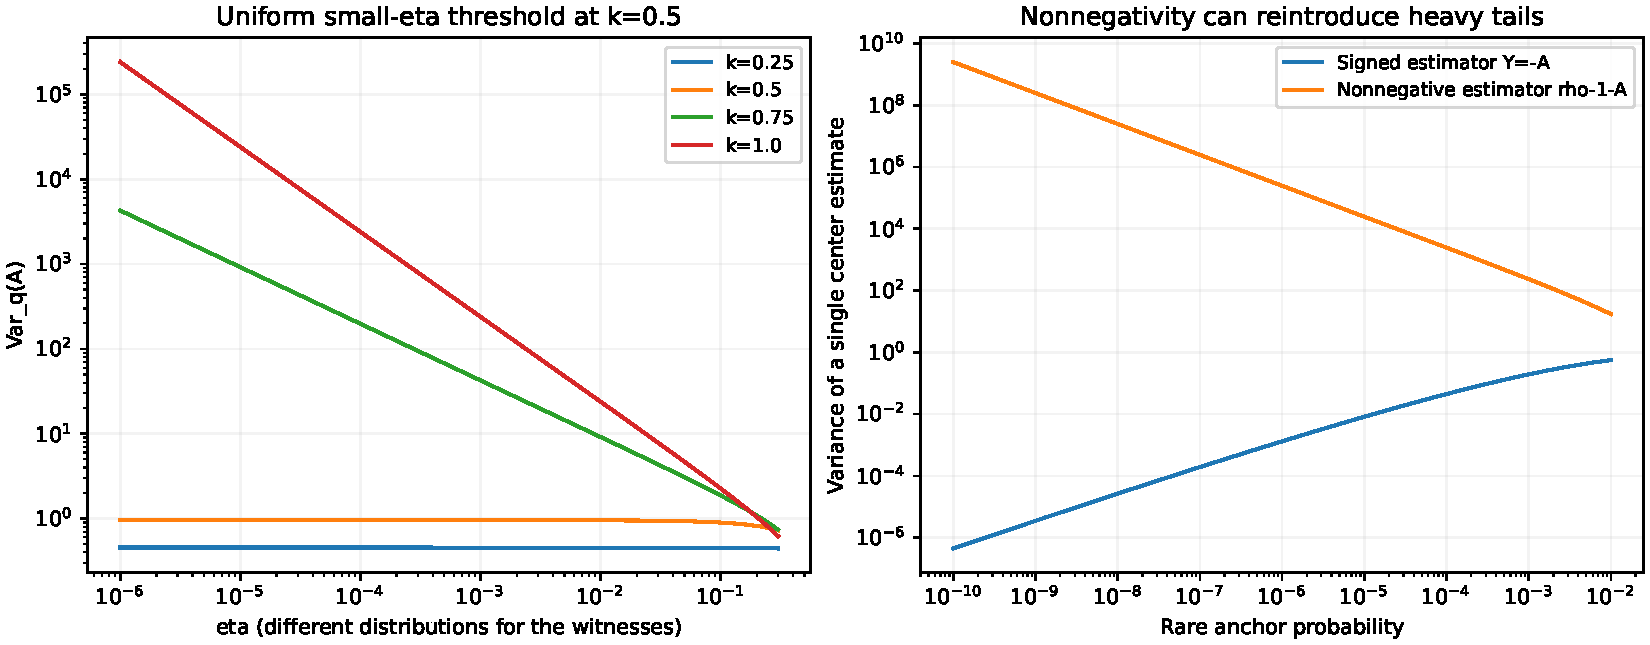
\includegraphics[width=\textwidth]{../../results/power-center-advantage/small-step-and-estimation.pdf}
 \caption{左：小步方差阈值的下界见证，不同形状使用不同分布族，不能当作同数据上的性能排名。右：逐样本非负中心估计可能重新引入概率比重尾。}
\end{figure}
\begin{figure}[htbp]
 \centering
 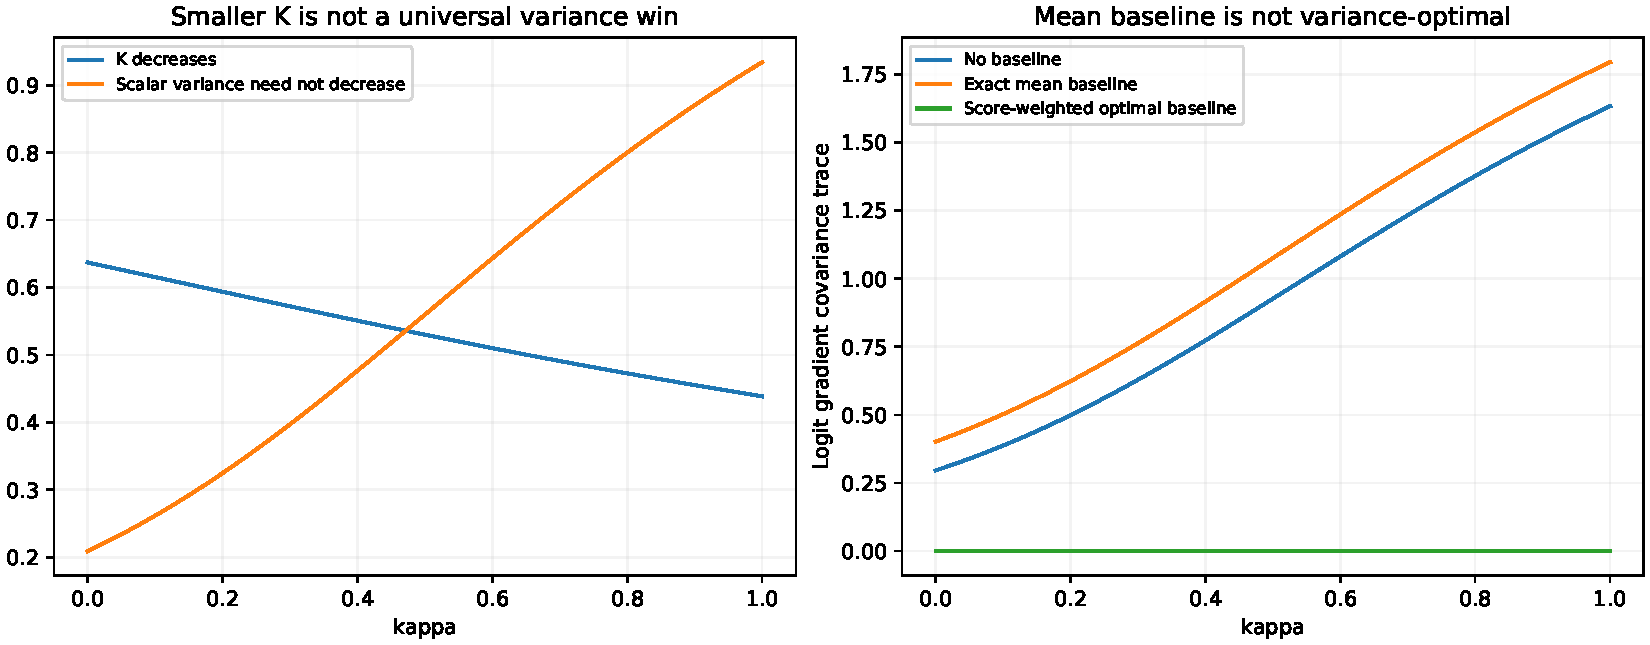
\includegraphics[width=\textwidth]{../../results/power-center-advantage/baseline-counterexample.pdf}
 \caption{同一二元输入下，$K$ 随形状下降但标量方差不必下降；均值 baseline 也不一定降低 logit 梯度方差。零方差最优 baseline 是二元例子的性质，不是一般网络结论。}
\end{figure}

数学核验与真实缓存审计见 \path{experiments/analysis/power_center_advantage.py}；真实缓存取原 64 条 t22 response 每条两个固定随机 reservoir 位置，共 128 个 prefix，对 20 组 $\kappa,\eta$ 精确求 action 条件矩。结果与所有实验统一维护在唯一实验报告；这些 CPU 模型分布统计不等于新 GPU 训练或全参数梯度方差。
